\documentclass{report}

\newcommand{\organization}{\textit{Arukana}}
\newcommand{\name}{\textit{Arcana Azurea Pitou}}
\newcommand{\program}{\textit{neko}}
\newcommand{\dependency}{\textit{editeur}}

\usepackage[french]{babel}
\usepackage[T1]{fontenc}
\usepackage[utf8]{inputenc}
\usepackage{fontspec}
\usepackage[a4paper]{geometry}
\usepackage{scrextend}
\usepackage{listings}
\usepackage[hidelinks,unicode=true]{hyperref}
\usepackage[pgf]{dot2texi}
\usepackage{pgf}
\usepackage{tikz}
\usepackage{fancyhdr}
\usepackage{sectsty}
\usepackage{titlesec}
\usepackage{csquotes}
\usepackage{hyperref}
\usepackage{keystroke}
\usepackage{booktabs}
\usepackage{color, colortbl}
\usepackage[labelformat=empty]{caption}
\usepackage{framed}
\usepackage[linguistics]{forest}

\hypersetup{
  colorlinks = true,
  linkcolor = blue,
  urlcolor = blue,
}

\usetikzlibrary{automata}

\pagestyle{fancy}

\fancyhf{}
\lhead{\leftmark}
\rhead{\rightmark}
\rfoot{\thepage}

\setmainfont[
    Path = fonts/sazanami-neko/,
    Extension = .ttf,
    Ligatures = TeX,
    Scale = MatchLowercase,
]{sazanami-mincho}

\setsansfont[
    Path = fonts/sazanami-neko/,
    Extension = .ttf,
    Ligatures = TeX,
    Scale = MatchLowercase,
]{sazanami-gothic}

\title{"neko"}

\author{
   adjivas
   \and
   brezaire
   \and
   flime
   \and
   jpepin
}

\date{}

\begin{document}

\begin{titlepage}
	\centering
	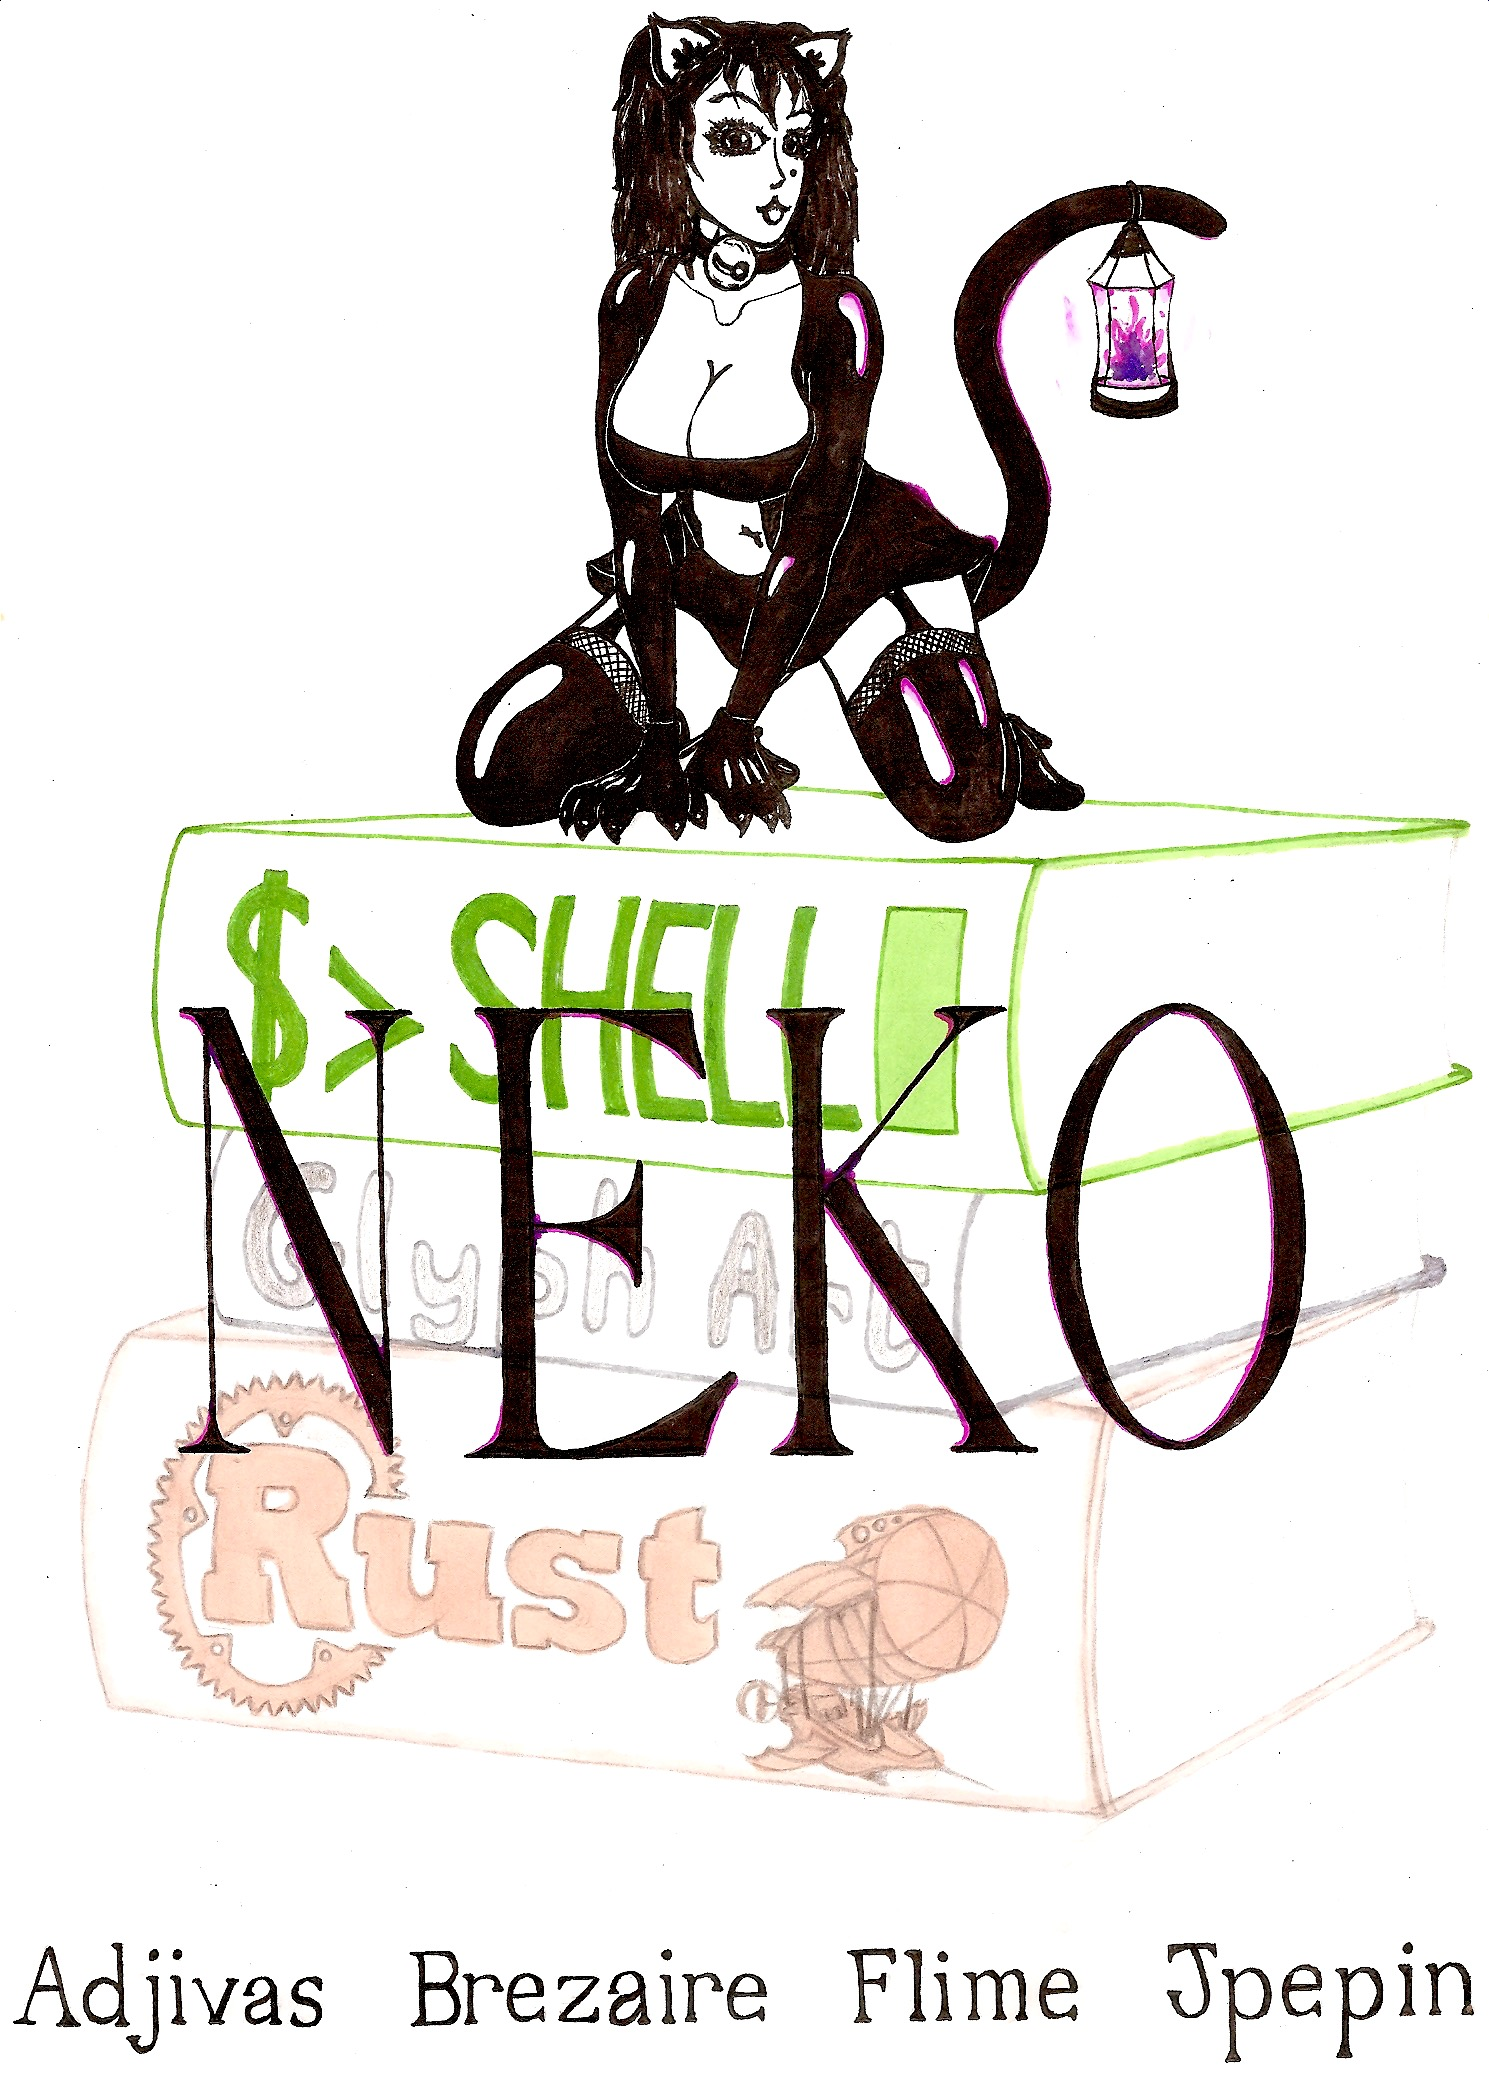
\includegraphics[scale=0.25]{images/neko.jpg}
\end{titlepage}

\tableofcontents

\titleformat{\chapter}[display]
  {\Huge}
  {\filleft\texttt{\chaptertitlename} \Huge\thechapter}
  {0ex}
  {\filleft}
  [\titlerule]

\chapter{Premiere partie}

\section{Préambule}

\begin{figure}[!ht]
  \begin{minipage}{1in}
    \centering
    \fontsize{30pt}{7pt}\selectfont
    \symbol{"E000}\symbol{"E001}\symbol{"E002}\symbol{"E003}\symbol{"E004}\symbol{"E005}\symbol{"E006}\symbol{"E007}\symbol{"E008}\symbol{"E009}\\*
    \symbol{"E00A}\symbol{"E00B}\symbol{"E00C}\symbol{"E00D}\symbol{"E00E}\symbol{"E00F}\symbol{"E010}\symbol{"E011}\symbol{"E012}\symbol{"E013}\\*
    \symbol{"E014}\symbol{"E015}\symbol{"E016}\symbol{"E017}\symbol{"E018}\symbol{"E019}\symbol{"E01A}\symbol{"E01B}\symbol{"E01C}\symbol{"E01D}\\*
    \symbol{"E01E}\symbol{"E01F}\symbol{"E020}\symbol{"E021}\symbol{"E022}\symbol{"E023}\symbol{"E024}\symbol{"E025}\symbol{"E026}\symbol{"E027}\\*
    \symbol{"E028}\symbol{"E029}\symbol{"E02A}\symbol{"E02B}\symbol{"E02C}\symbol{"E02D}\symbol{"E02E}\symbol{"E02F}\symbol{"E030}\symbol{"E031}\\*
  \end{minipage}
  \caption[Caption for LOF]{\href{https://en.wikipedia.org/wiki/Wikipedia:Wikipe-tan}{Wikipe-tan} \textendash{ ウィキペたん }\textendash{ }}
\end{figure}

Une nékoe \textendash{ ねこみみ }\textendash{ } est un persona d'animé japonais avec des traits de chat
\textendash{ mimikko
	\footnote{ Kemonomimi ou mimikko est un personnage humain d'animé avec les caractéristiques d'un animal telles que sa personnalité ou encore son physique
		\textendash{ 獣耳 }\textendash.
			}} \textendash.

Le GlyphArt est l'écriture d'une image via des caractères compris dans l'Unicode privé, ce projet démontre ce procédé via
\href{https://limaconoob.github.io/Image2font}{Image2font}.

$\name$ est une programmeuse nékoe fictive de terminal inventée pour assister des utilisateurs.

\section{Introduction}
\thispagestyle{empty}
$\name$ est une nékoe de terminal qui a pour but d'apporter les Arts, la Culture et une assistance à qui saura utiliser un shell.
Humanisée d’émotions et fondée sur l'expérience de la \href{https://fr.wikipedia.org/wiki/Chambre_chinoise}{chambre chinoise}, celle-ci sera donc instruite via des bibliotèques.

L'organisation GitHub $\organization$ de philosophie \href{https://fr.wikipedia.org/wiki/Libriste}{libriste} fut créée pour distribuer et maintenir communautairement les dépôts nécessaires au développement d'une Nékoe de terminal.


\begin{figure}[!ht]
    \begin{minipage}{\textwidth}
    \centering
		\begin{tabular}{p{.10\textwidth}p{.90\textwidth}}
			\textbf{\href{https://github.com/Arukana/book/tree/documentation}{Book}} & La documentation du projet $\program$. \\
            \textbf{\href{https://github.com/Arukana/PtyProc}{PtyProc}} & L'\href{https://fr.wikipedia.org/wiki/Middleware}{intergiciel} \textendash{ \href{https://en.wikipedia.org/wiki/Middleware}{Middleware} }\textendash{ } et l'\href{https://fr.wikipedia.org/wiki/Backend}{arrière-plan} \textendash{ back-end  }\textendash{ } de l'émulateur du terminal \href{https://fr.wikipedia.org/wiki/VT100}{VT100}. \\
            \textbf{\href{https://github.com/Arukana/Editor}{Editor}} & L'éditeur et la bibliothèque d'expression de la nékoe. \\
            \textbf{\href{https://github.com/Arukana/Neko.git}{Neko}} & Le programme $\program$. \\
            \textbf{\href{https://github.com/Arukana/LibNya.git}{LibNya}} & La bibliothèque dynamique de teste du programme $\program$. \\
            \textbf{\href{https://github.com/Arukana/ffi.git}{ffi}} & L'\href{https://fr.wikipedia.org/wiki/Header}{en-têtes} \textendash{ \href{https://en.wikipedia.org/wiki/Header_(computing)}{header} }\textendash{ } sont les déclarations des structures et énumérations de la nékoe. \\
	        \textbf{\href{https://github.com/Arukana/Image2font}{Image2font}} & Le convertisseur d'images en une police d’écriture. \\
            \textbf{\href{https://github.com/Arukana/nTerm}{nTerm}} & L'\href{https://fr.wikipedia.org/wiki/Interface_graphique}{interface graphique} de émulateur. \\
        \end{tabular}
		\caption*{
			\begin{forest}
			    [Terminal
					[Neko
					    [Editeur]
                        [PtyProc
						    [Pty]
					    ]
					]
			    ]
			\end{forest}
		}
    \end{minipage}
\end{figure}

\subsection{Utilisation}

La constante d’environnement textit{NEKO\_PATH} pourra être définit à \enquote{HOME/.neko} et comprendra les sous-répertoires \textit{lib}, \textit{rep}, \textit{texel} et \textit{sprite}. Sinon, les href{https://fr.wikipedia.org/wiki/Biblioth%C3%A8que_logicielle}{bibliothèques} de l'organisation $\name$ ceux reporterons à constante \textit{CARGO_MANIFEST_DIR} de valeurs relatives aux répertoires contenant les \href{https://en.wikipedia.org/wiki/Manifest_file}{fichiers manifests}.

\subsubsection{Programme $\program$ \textendash{\href{https://fr.wikipedia.org/wiki/Interface_en_ligne_de_commande}{CLI}}\textendash{}}

\begin{figure}[!ht]
    \begin{minipage}{\textwidth}
    \centering
        \begin{tabular}{p{.15\textwidth}p{.20\textwidth}p{.65\textwidth}}
                \textbf{\textendash\textendash help} && Imprime ce menu d'aide \\
                \textbf{\textendash\textendash version, \textendash{V}} && Imprime la version du programme $\program$ \\
                \textbf{\textendash\textendash command, \textendash{c}} & [/bin/zsh] & Précise le processus fils. \\
                \rowcolor{yellow}
                \textbf{\textendash\textendash repeat, \textendash{r}} & [1000] & Précise le temps de répétition du maintien d'une touche enfoncée tel que $\{2\dots{}N\}$. \\
                \rowcolor{yellow}
                \textbf{\textendash\textendash interval, \textendash{i}} & [1000] & Précise le temps d'intervalle durant les répétitions tel que $\sum_{i=repeat}^{\infty} U_{interval}\times{}i$. \\
        \end{tabular}
    \end{minipage}
    \caption[Caption]{ \colorbox{yellow}{\phantom{\_}} Fonctionnalité supplémentaire \enquote{keyboard-time}.}
\end{figure}

%\subsection{\href{https://fr.wikipedia.org/wiki/Interpr%C3%A8te_(informatique)}{Interpréteur}}

\subsubsection{Commande $\program$ \textendash{\href{https://en.wikipedia.org/wiki/Shell_builtin}{builtin}\textendash{}}}

Le programme $\program$ substitura la commande \enquote{neko}(1) pour et uniquement pour son processus enfant qui sera à l'occurrence notre \href{https://fr.wikipedia.org/wiki/Interpr%C3%A9teur_de_commandes}{d'interprétation de commandes}. \\

Cette commande comprend les options si-suivantes: \\

\begin{figure}[!ht]
    \begin{minipage}{\textwidth}
    \centering
		\begin{tabular}{p{.30\textwidth}p{.16\textwidth}p{.54\textwidth}}
			\textbf{install <url>} & https://git... & Installe depuis dépôt distant un plugiciel. \\
			\textbf{uninstall <author@libname>} & Arukana@LibNya & Désinstalle les sources et la bibliothèque dynamique d'un plugiciel \textendash{} \href{https://fr.wikipedia.org/wiki/Plugin}{plugin} \textendash{}. \\
			\textbf{mount <author@libname> [<priority>]} & Arukana@LibNya 1 & Monte une bibliothèque dynamique avec une priorité de niveau zero. \\
			\textbf{unmount <author@libname>} & Arukana@LibNya & Démonte une bibliothèque dynamique. \\
			\textbf[\textbf{update <author@libname>}] & Arukana@LibNya & Révise une bibliothèque dynamique. \\
		\end{tabular}
    \end{minipage}
\end{figure}

\subsection{Interface de fonctions dynamiques \textendash{\href{https://en.wikipedia.org/wiki/Foreign_function_interface}{FFI}}\textendash{}}

\begin{figure}[!ht]
    \begin{minipage}{\textwidth}
    \centering
        \begin{tabular}{p{.50\textwidth}p{.50\textwidth}}
            \textbf{void start\(t_lbstat *state, void **save\)} & Imprime ce menu d'aide \\
        \end{tabular}
    \end{minipage}
%    \caption[Caption]{ \colorbox{yellow}{\phantom{\_}} Fonctionnalité supplémentaire \enquote{keyboard-time}.}
\end{figure}

\section{$\dependency$}

 est l'interface d'une liste de primitives telles que des texels et des sprites qui pourront se combiner en nouveaux sprites. \\

L'$\dependency$ est à la fois : \\

\begin{enumerate}
	\item Un programme qui selon une liste de primitive permettra de devirer des expressions en commandes.
	Interface utilisateur en mode texte -\href{https://en.wikipedia.org/wiki/Text-based_user_interface}{TUI}-.
	\item Une bibliothèque et dépenpence du projet Neko, qui chargera un dictionnaire de \href{https://fr.wikipedia.org/wiki/Sprite_(jeu_vid%C3%A9o)}{lutin} -\href{https://en.wikipedia.org/wiki/Sprite_(computer_graphics)}{sprite}-.
\end{enumerate}

\subsection{Programme \href{https://en.wikipedia.org/wiki/Text-based_user_interface}{\textendash{TUI}\textendash{}}}

L'$\dependency$ comprend une liste d'animation, de un à seize sprites chacuns. Un sprite sera derivé selon des groupes d'émotions, formant ainsi une multitude expressions. La somme des sprites représente la configuration d'une animation. \\*

\begin{tabbing}
    Quit <q> \\*
    bust \\*
    0 - PT0.200S: Talk \\*
    \symbol{"E000}\symbol{"E001}\symbol{"E002}\symbol{"E003}\symbol{"E004}\symbol{"E005}\symbol{"E006}\symbol{"E007}\symbol{"E008}\symbol{"E009} HeHeHe\_\_\_\_\_\_\_\_\_\_\_\_\_\_ \_\_\_\_\_\_\_\_\_\_ \\*
    \symbol{"E00A}\symbol{"E00B}\symbol{"E00C}\symbol{"E00D}\symbol{"E00E}\symbol{"E00F}\symbol{"E010}\symbol{"E011}\symbol{"E012}\symbol{"E013} HeHeHe\_\_\_\_\_\_\_\_\_\_\_\_\_\_ \_\_\_\_\_\_\_\_\_\_ \\*
    \symbol{"E014}\symbol{"E015}\symbol{"E016}\symbol{"E017}\symbol{"E018}\symbol{"E019}\symbol{"E01A}\symbol{"E01B}\symbol{"E01C}\symbol{"E01D} \_\_\_\_\_\_\_\_Mo\_\_\_\_\_\_\_\_\_\_ \_\_\_\_\_\_\_\_\_\_ \\*
    \symbol{"E01E}\symbol{"E01F}\symbol{"E020}\symbol{"E021}\symbol{"E022}\symbol{"E023}\symbol{"E024}\symbol{"E025}\symbol{"E026}\symbol{"E027} \_\_\_\_\_\_\_\_\_\_\_\_\_\_\_\_\_\_\_\_ \_\_\_\_\_\_\_\_\_\_ \\*
    \symbol{"E028}\symbol{"E029}\symbol{"E02A}\symbol{"E02B}\symbol{"E02C}\symbol{"E02D}\symbol{"E02E}\symbol{"E02F}\symbol{"E030}\symbol{"E031} \_\_\_\_\_\_\_\_\_\_\_\_\_\_\_\_\_\_\_\_ \_\_\_\_\_\_\_\_\_\_ \\*
    \\*
    S\_ \\*
    1 - PT0.200S: NotTalk \\*
    \symbol{"E000}\symbol{"E001}\symbol{"E002}\symbol{"E003}\symbol{"E004}\symbol{"E005}\symbol{"E006}\symbol{"E007}\symbol{"E008}\symbol{"E009} HeHeHe\_\_\_\_\_\_\_\_\_\_\_\_\_\_ SSS\_\_\_\_\_\_\_ \\*
    \symbol{"E00A}\symbol{"E00B}\symbol{"E00C}\symbol{"E00D}\symbol{"E00E}\symbol{"E00F}\symbol{"E010}\symbol{"E011}\symbol{"E012}\symbol{"E013} HeHeHe\_\_\_\_\_\_\_\_\_\_\_\_\_\_ SSS\_\_\_\_\_\_\_ \\*
    \symbol{"E014}\symbol{"E015}\symbol{"E016}\symbol{"E017}\symbol{"E018}\symbol{"E019}\symbol{"E01A}\symbol{"E01B}\symbol{"E01C}\symbol{"E01D} \_\_\_\_\_\_\_\_Mo\_\_\_\_\_\_\_\_\_\_ \_\_\_\_\_\_\_\_\_\_ \\*
    \symbol{"E01E}\symbol{"E01F}\symbol{"E020}\symbol{"E021}\symbol{"E022}\symbol{"E023}\symbol{"E024}\symbol{"E025}\symbol{"E026}\symbol{"E027} \_\_\_\_\_\_\_\_\_\_\_\_\_\_\_\_\_\_\_\_ \_\_\_\_\_\_\_\_\_\_ \\*
    \symbol{"E028}\symbol{"E029}\symbol{"E02A}\symbol{"E02B}\symbol{"E02C}\symbol{"E02D}\symbol{"E02E}\symbol{"E02F}\symbol{"E030}\symbol{"E031} \_\_\_\_\_\_\_\_\_\_\_\_\_\_\_\_\_\_\_\_ \_\_\_\_\_\_\_\_\_\_ \\*
    \\*
    \_S \\*
    --Talk --NotTalk Heart:Shocked \\*
\end{tabbing}

\subsubsection{Raccourcis clavier}

La saisie est adapté selon la disposition des touches du \href{https://en.wikipedia.org/wiki/ADM-3A}{terminal ADM-3A} de la société \href{https://en.wikipedia.org/wiki/Lear_Siegler}{Lear Siegler}.

\begin{figure}[!ht]
  \begin{minipage}{\textwidth}
    \centering
    \begin{tabular}{p{.3\textwidth}p{.7\textwidth}}
        \toprule
        \toprule
            Touche & Description \\
        \midrule
            \Ctrl+\keystroke{q}ou\keystroke{q} & Quitter le programme. \\
            \rowcolor{yellow}
            \Ctrl+\keystroke{c}ou\keystroke{c} & Copier la commande dans le presse-papier. \\
            \Home{}ou\keystroke{g} & Sélectionner la première animation. \\
            \PgUp{}ou\keystroke{H} & Sélectionner l'animation précédente. \\
            \PgDown{}ou\keystroke{L} & Sélectionner l'animation suivante. \\
            \End{}ou\keystroke{G} & Sélectionner la dernière animation. \\
            \keystroke{\{}ou\keystroke{[} & Sélectionner le sprite précédent. \\
            \keystroke{\}}ou\keystroke{]} & Sélectionner le sprite suivant. \\
            \LArrow{}ou\keystroke{h} & Sélectionner la cellule de gauche. \\
            \UArrow{}ou\keystroke{k} & Sélectionner la cellule du haut. \\
            \DArrow{}ou\keystroke{j} & Sélectionner la cellule du bas. \\
            \RArrow{}ou\keystroke{l} & Sélectionner la cellule de droite. \\
            \keystroke{0}...\keystroke{9} & Changer la cellule courrante. \\
        \bottomrule
    \end{tabular}
  \end{minipage}
  \caption[Caption]{ \colorbox{yellow}{\phantom{\_}} Fonctionnalité supplémentaire \enquote{Clipboard}.}
\end{figure}

\subsubsection{Bibliothèque}

\footnotetext{En génie logiciel, le langage de modélisation orienté objet unifié de l'anglais
	\enquote{Unified Modeling Language}
		\textendash{ UML }\textendash{ } est la représentation schématique d'un programme par de l'orienté objet}

\begin{figure}[!ht]
  \centering
  \begin{dot2tex}[dot,scale=0.25]
digraph graphic {
  d2tstyleonly = true;
  node [shape = "box", width = "2.5", texmode="verbatim", style = "top color=cyan!10,bottom color=cyan!35,draw=cyan!50,rounded corners"];
  graph [shape = "box", texmode="math", style = "top color=blue!10,bottom color=blue!35,draw=blue!50"];

  nodeGraphic [label="Struct Graphic<Default + Debug + Clone>\n
    texel: HashMap<Posture, HashMap<Tuple, Vec<Texel>>>,
    sprite: io::Cursor<Vec<(Sheet, Sprite)>>,
  "];

  nodeTuple [label="Struct Tuple<Copy + Clone + Debug + Default + Eq + PartialEq + Hash + From>\n
    + Part,
    + Emotion,
  "];

  nodeDraw [label="Struct Draw<Default + Debug + Clone + IntoIterator>\n
    posture: Posture,
    duration: time::Duration,
    board: io::Cursor<[(Emotion, Texel); SPEC_MAX_XY]>,
  "];

  nodeTexel [label="Struct Texel<Default + Copy + Clone + Display + Debug + PartielEq>\n
    part: Part,
    glyph: char,
  "];

  nodeSprite [label="Struct Sprite<Default + Clone + IntoIterator>\n
    texel: HashMap<Tuple, Vec<Texel>>,
    sheet: io::Cursor<[Draw; SPEC_MAX_DRAW]>,
    count: usize,
  "];

  nodePart [label="Enum Part<Default + Display + Debug + Clone + Copy + Eq + PartialEq + Hash>\n
    None = b'_',
    ArmLeft = b'a',
    ArmRight = b'A',
    Boobs = b'b',
    Clavicle = b'c',
    EarLeft = b'e',
    EarRight = b'E',
    EyeLeft = b'y',
    EyeRight = b'Y',
    HairTop = b'o',
    HairLeft = b'r',
    HairRight = b'R',
    HandLeft = b'd',
    HandRight = b'D',
    Mouth = b'm',
    Tail = b't',
    Bell = b'l',
    ExclamationMark = b'x',
    ExclamationMarks = b'X',
    Heart = b'h',
    Hearts = b'H',
    Lantern = b'n',
    QuestionMark = b'q',
    QuestionMarks = b'Q',
    WoolBall = b'w',
  "];

  nodePosture [label="Enum Posture<Default + Display + Debug + Clone + Copy + Eq + PartialEq + Hash>\n
    None = b'_',
    Talk = b't',
    NotTalk = b'n',
    Bust = b'b',
    Lying = b'l',
    Seiza = b's',
  "];

  nodeSheet [label="Enum Sheet<Default + Display + Debug + Clone + Copy + Eq + PartialEq + Hash>\n
    None = b'_',
    Bust = b'b',
  "];

  nodeEmotion [label="Enum Emotion<Default + Display + Debug + Clone + Copy + Eq + PartialEq + Hash>\n
    None = b'_',
    Angry = b'a',
    Happy = b'h',
    Love = b'l',
    Malicious = b'm',
    Misunderstanding = b'i',
    Shocked = b'o',
    Sleepy = b's',
	Speechless = b'e',
  "];

  nodePosture -> nodeGraphic;
  nodeTuple -> nodeGraphic;
  nodeTexel -> nodeGraphic;
  nodeSheet -> nodeGraphic;
  nodeSprite -> nodeGraphic;
  nodeTexel -> nodeSprite;
  nodeDraw -> nodeSprite;
  nodePart -> nodeTexel;
  nodePart -> nodeTuple;
  nodeEmotion -> nodeTuple;
  nodePosture -> nodeDraw;
  nodeTexel -> nodeDraw;
  nodeEmotion -> nodeDraw;
}
  \end{dot2tex}
  \caption[Caption for LOF]{ Diagramme UML \footnotemark{} simplifié du module graphique. }
  \label{graphic}
\end{figure}

\end{document}
